\zexternaldocument{evaluatie}
\zexternaldocument{inleiding}

\chapter{Analyse van het probleem}
\label{sec:analyse}
Door zo veel mogelijk afhankelijkheden uit het configuratiemodel te halen kan een grote tijdswinst behaalt worden tijdens het uitrollen van dat model.
Als de CMS beschikt over alle bestaande afhankelijkheden kan ze namelijk in \'e\'en keer het volledige model correct uitrollen.
Het doel is dus om niet alleen de afhankelijkheden te gebruiken die expliciet vermeld staan maar ook heuristieken te gebruiken om impliciete afhankelijkheden af te leiden.

Deze heuristieken worden toegepast eens het model volledig opgesteld en voordat het uitrollen begint.
Zo beschikken ze over alle nodige informatie en kan nog extra informatie toegevoegd worden aan het model.
Deze orde waarin deze heuristieken opgeroepen worden kan vastgelegd worden. Dit komt handig van pas bij het verwerken van relaties in het model, zie sectie \ref{sec:relaties} en \ref{sec:hoog_niveau_relaties}.

\section{Afhankelijkheden tussen bestanden en mappen}
\label{sec:bestanden_en_mappen}
Tussen bestanden en mappen bestaat er zonder twijfel een sterke afhankelijkheid: een bestand kan helemaal niet bestaan zonder een map.
Visueel is dit voorgesteld in figuur \ref{fig:file_dir_dep}.
De eerste heuristiek die werd ontwikkeld voor IMP is er een die voor elk bestand de bijhorende map opzoekt in het model en een afhankelijkheid toevoegd als deze gevonden wordt.
Het algoritme dat hiervoor gebruikt wordt ziet eruit als volgt (pseudocode):

\begin{minipage}{\textwidth}
\begin{lstlisting}[language=Python]
foreach file in resources:
    foreach dir in resources:
        if get_directory(file.path) == dir.path:
            file.requires.append(dir)
\end{lstlisting}
\end{minipage}

Als de map niet vermeld wordt in het model wordt deze ook niet toegevoegd omdat dit ongewenste gevolgen kan hebben. \todo{Welke?}

\section{Afhankelijkheden tussen services, packages en configuratiebestanden}
\label{sec:services_packages_en_configuratiebestanden}
Net zoals tussen bestanden en mappen is er een sterke afhankelijkheid tussen packages, services en hun eventuele configuratiebestanden:
een service kan niet gestart worden als zijn package niet ge\"installeerd is en zal niet correct werken zonder een aangepast configuratiebestand.
Een grafische voorstelling hiervan is te vinden op figuur \ref{fig:service_package_dep}.

\begin{figure}[h]
    \begin{center}
    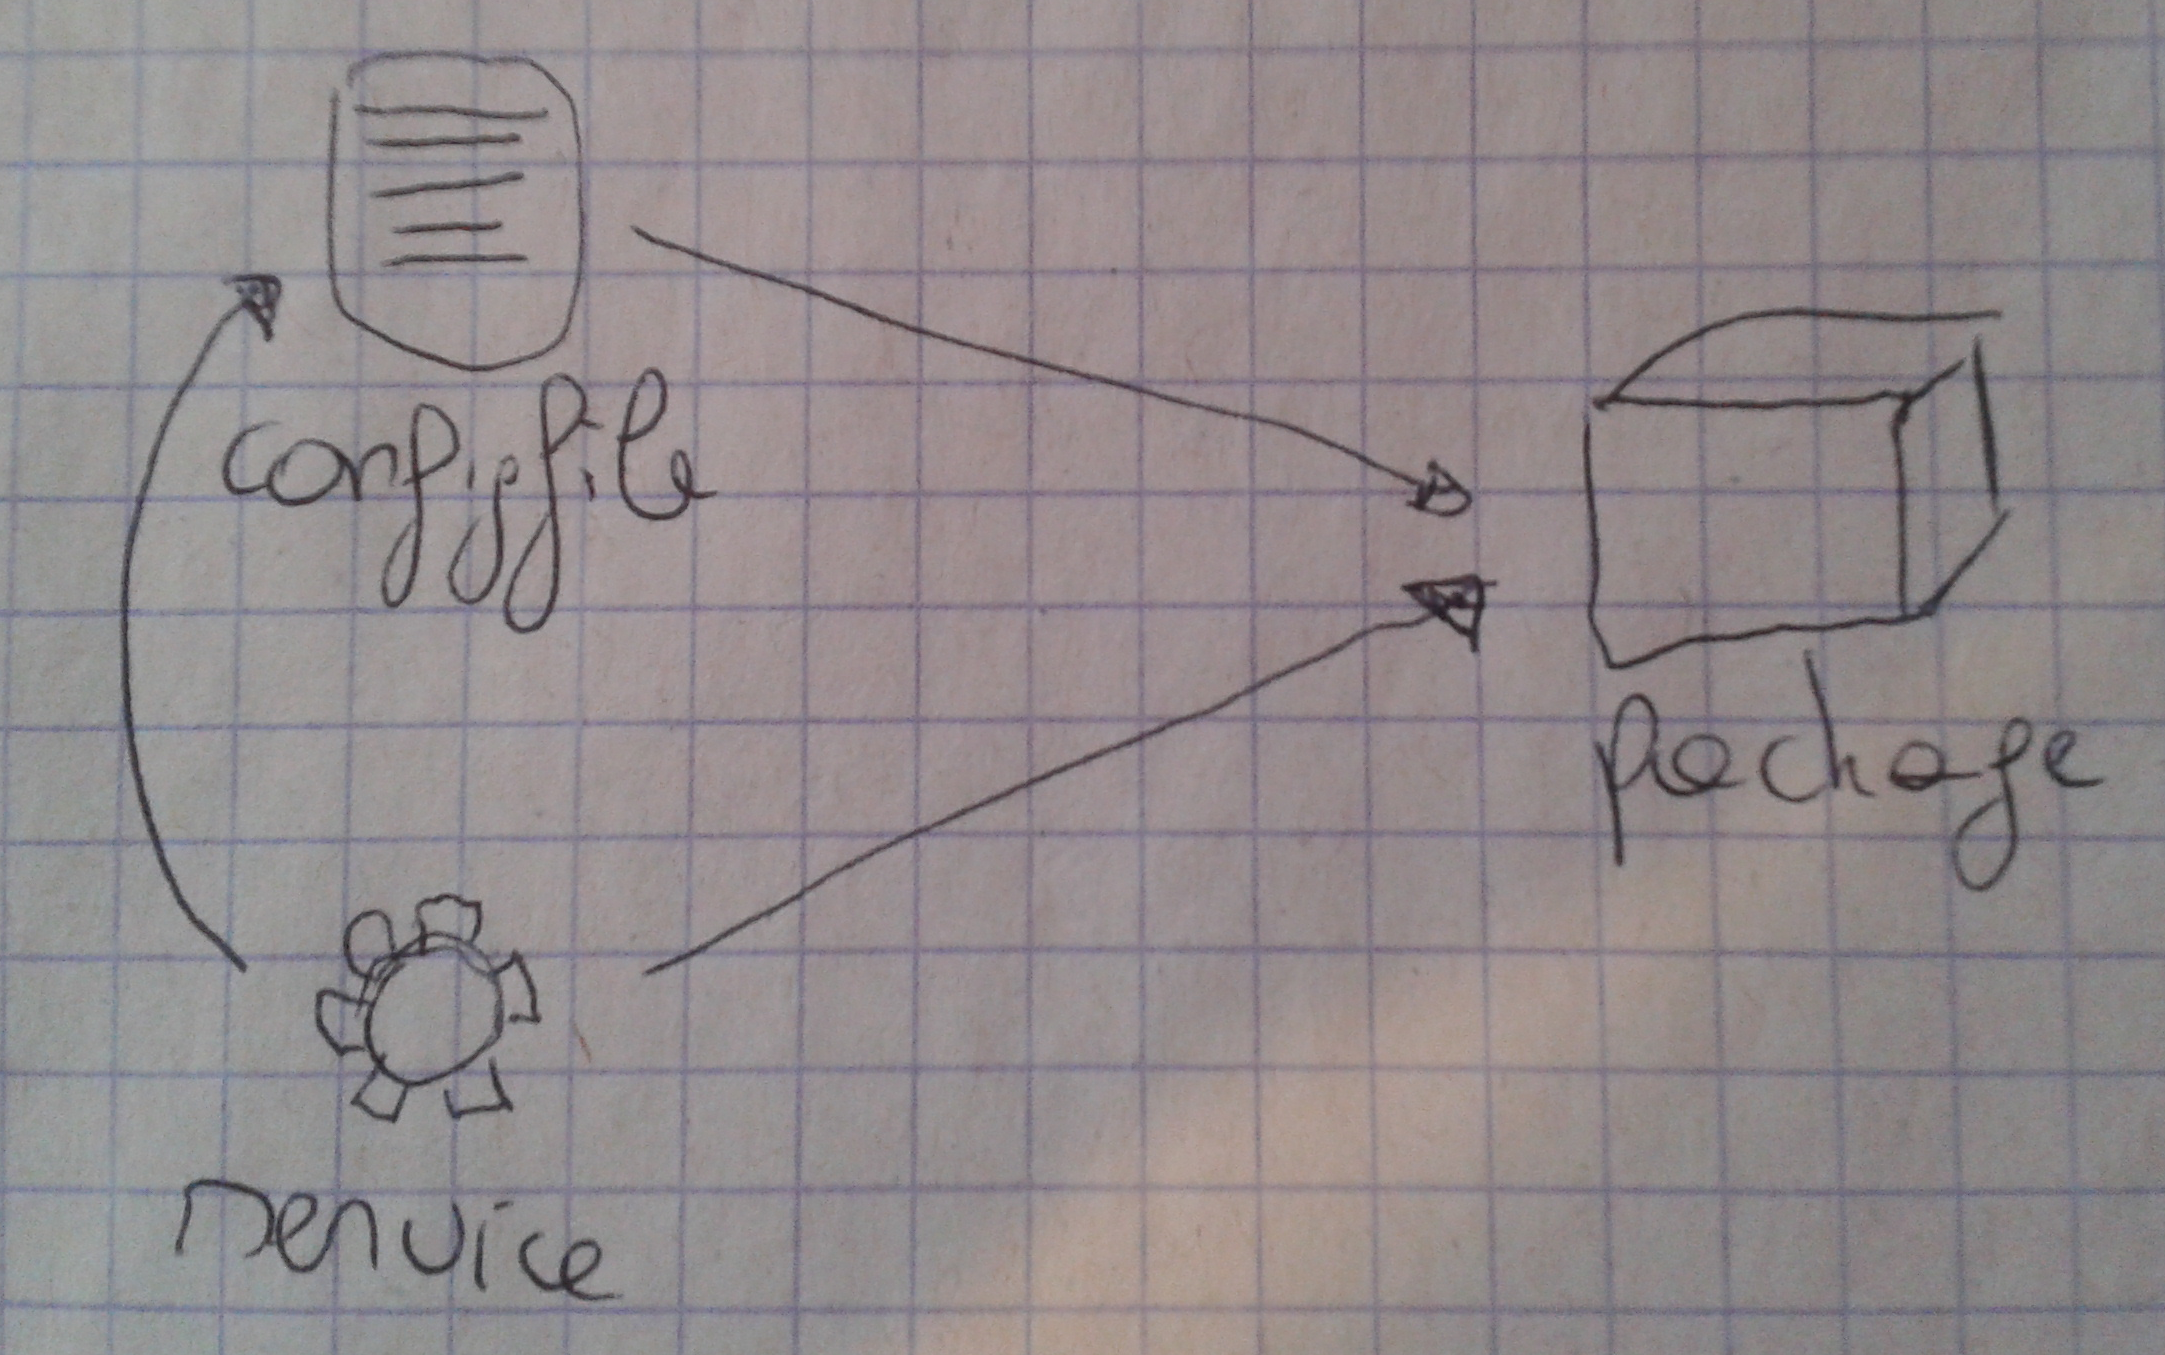
\includegraphics[width=0.6\textwidth]{images/service_package_dep.png}
    \caption{Grafische voorstelling van de afhankelijkheden die voorkomen tussen packages, services en configuratiebestanden}
    \label{fig:service_package_dep}
    \end{center}
\end{figure}

De meest simplistische aanpak om de correcte afhankelijkheden te introduceren is alle services afhankelijk maken van alle packages en files en alle files afhankelijk van de packages.
De configuratiebestanden mogen pas geplaatst worden nadat de packages ge\"installeerd zijn omdat anders het aangepast configuratiebestand overschreven wordt.
Dit introduceert uiteraard veel afhankelijkheden die niet overeenstemmen met de werkelijkheid maar ze maken daardoor het resultaat van het uitrolproces niet fout.
Een algoritme in pseudocode ziet er uit als volgt:

\begin{minipage}{\textwidth}
\begin{lstlisting}[language=Python]
foreach service in resources:
    foreach file in resources:
        service.requires.append(file)
    foreach package in resources:
        service.requires.append(package) foreach file in resources:
		foreach package in resources:
				file.requires.append(package)
\end{lstlisting}
\end{minipage}

De volgende aanpak gebruikt wat meer info uit het model en resulteert in minder overbodige afhankelijkheden.
In de modelcode worden bestanden, packages en services die bij elkaar horen meestal binnen eenzelfde implementatie gespecifi\"eerd.
Een voorbeeld is de implementatie van een MySQL server:

\begin{minipage}{\textwidth}
\begin{lstlisting}
implementation mysql:
    pkg = std::Package(host= host, name= "mysql-server", state= "installed")
    svc = std::Service(host= host, name= "mysqld", state= "running", onboot= true)

    config= std::ConfigFile(host= host, path= "/etc/my.cnf", content= template("mysql/my.cnf.tmpl"), requires= pkg, reload= true)
    conf_dir= std::Directory(host= host, path= "/etc/mysql.conf.d", owner= "root", group= "root", mode= 755)

    dblist= std::ConfigFile(host= host, path= "/etc/sysconfig/mysql", reload= true, content= template("mysql/databases.tmpl"))
end
\end{lstlisting}
\end{minipage}

Bij het verwerken van het model tijdens het uitrolproces bevinden al deze resources zich binnen dezelfde scope.
De heuristiek bestaat er uiteindelijk uit verzamelingen van packages en services te vinden die binnen \'e\'enzelfde scope gedefini\"eerd zijn en de correcte afhankelijkheden op te stellen tussen enkel die resources.
Deze verzamlingen worden "service stacks"  genoemd.
De aanwezigheid van files is optioneel: sommige servicen moeten niet verder geconfigureerd worden.
Algoritmisch ziet de code hiervoor  er uit als volgt (pseudocode):

\begin{minipage}{\textwidth}
\begin{lstlisting}
srv_stacks = []
for resource in resources:
    same_scope = [res in resources where res.scope == resources.scope]
    if same_scope.contains(services) and same_scope.contains(packages):
        srv_stacks.append(same_scope)

foreach stack in srv_stacks:
    foreach service in stack:
        foreach file in stack:
            service.requires.append(file)
        foreach package in stack:
            service.requires.append(package)
\end{lstlisting}
\end{minipage}

\section{Afhankelijkheden door relaties}
\label{sec:relaties}
IMP laat toe in het model relaties tussen concepten te specifi\"eren.
Een voorbeeldrelatie is de volgende:
\begin{lstlisting}
BaseClient clients [0:] -- [0:] BaseServer servers
\end{lstlisting}
Deze betekent dat een BaseClient nul of meerdere BaseServers nodig heeft, en omgekeerd.
Een ander voorbeeld is 
\begin{lstlisting}
Host host [1] -- [0:] File files
\end{lstlisting}
Deze betekent dat op een Host nul of meerdere files kunnen staan, maar dat elke File \'e\'en Host moet hebben.
Hieruit kunnen we afleiden dat een File niet kan bestaan zonder een host en het dus nodig is dat eerst de Host moet bestaan en opgestart zijn voordat geprobeerd wordt de File te cree\"eren.

Algemeen kan men dus besluiten dat elke relatie waar de ene kant een multipliciteit van [0] of [0:] heeft en de andere kant multipliciteit [1] of [1:] de eerste entiteit afhankelijk is van de tweede.
De code voor deze heuristiek ziet er uit als volgt:

\begin{minipage}{\textwidth}
\begin{lstlisting}
for lib in model.get_scopes():
    for concept in lib.variables():
        if concept.hasattr(relation)
            if concept.relation.low == 0 and concept.relation.end == 1:
                concept.relation.depends = True
\end{lstlisting}
\end{minipage}

Het gebruik van relaties zoals deze tussen de webserver en de databaseserver beperkt het aantal deployment runs die nodig zijn om een werkende infrastructuur te bekomen.
Als enkel deze heuristiek gebruikt wordt zal IMP niets veranderen aan het uitrolproces.
De extra informatie die toegevoegd wordt kan wel gebruikt worden door andere heuristieken.
Een voorbeeld hiervan is deze hieronder (sectie \ref{sec:hoog_niveau_relaties}) die toelaat afhankelijk zoals deze tussen de webserver en databaseserver te gebruiken voor een optimaler uitrolproces.

\section{Afhankelijkheden tussen hoog-niveau concepten}
\label{sec:hoog_niveau_relaties}
IMP laat niet alleen toe om afhankelijkheden tussen enkelvoudige concepten zoals bestanden, services,\ldots te specifi\"eren maar ook tussen samengestelde concepten zoals webservers, databaseservers,\ldots
Deze betekenen dat de ene kant niet zijn volledige functionaliteit kan aanbieden zonder de aanwezigheid van de andere kant.
Aangezien een server zijn functionaliteit aanbiedt aan de hand van een service en niet zijn configuratiebestanden en pakketten stelt de volgende heuristiek enkel afhankelijkheden op tussen de services binnen afhankelijke concepten.
Het is onnodig om alle resources van het ene concept te laten afhangen van alle resources van het andere concept, het zijn enkel de services die van belang zijn.

IMP laat toe om verschillende libraries te gebruiken (en zelf te defini\"eren) met daarin voorgedefinieerde concepten. 
Het algoritme begint met het doorzoeken van deze libraries naar concepten die services bevatten.
Dan kijkt het of dat concept afhankelijk is van een ander concept.
Als dit het geval is wordt gekeken of dat ander concept ook services bevat.
Zo ja stelt het algoritme de nodige afhankelijkheden op.

In pseudocode ziet dit er uit als volgt:

\begin{minipage}{\textwidth}
\begin{lstlisting}
for lib in model:
    for concept in lib.variables():
        concept_services = get_services(concept)
        if concept_services is not None:
            for relation in concept.get_attributes():
                if relation.depends: #afhankelijke relatie
                    for instance in concept.values: #Voor elke instantie v/h concept
                        req_concepts = relation.end
                        req_resources = []
                        for req_concept in req_concepts:
                                for srv in get_services(req_concept):
                                    req_resources.append(srv)
                        if req_resources is not None: 
                            for service in concept_services:
                                for req_res in req_resources:
                                    service.requires.add(req_res)
\end{lstlisting}
\end{minipage}

Het is belangrijk dat deze heuristiek wordt opgeroepen na deze van sectie \ref{sec:relaties}, daar worden namelijk extra afhankelijke relaties opgesteld die hier kunnen gebruikt worden.

Deze heuristiek optimaliseert het uitrolproces op een andere manier dan de vorige.
Die zorgden er namelijk voor dat elke resource \emph{kon} uitgerold worden.
Het probleem is dat zelfs als elke resource correct uitgerold wordt de infrastructuur mogelijks nog altijd niet volledig werkt omdat sommige instanties niet in de juiste volgorde gestart werden.
Deze heuristiek probeert te garanderen dat wel de juiste volgorde gevolgd wordt.

\section{Besluit van dit hoofdstuk}

besluit

